% !TeX encoding = UTF-8

\chapter{INTRODUÇÃO}\label{ch:introducao}

Redes sociais se tornaram um termo comum e uma chave fundamental para o estilo de vida moderno. Hoje em dia, ....


\section{JUSTIFICATIVA}\label{sec:justificativa}
A rede social \textit{Twitter} é um excelente ponto de partida para a mineração de dados em redes sociais, ....

A rede social possui um total de 289 milhões de usuários ativos no mundo inteiro, totalizando 58 milhões de \textit{tweets} por dia \cite{statistics}.


\section{OBJETIVOS}\label{sec:objetivos}

\subsection{Objetivo Geral} 
Este trabalho tem como objetivo principal utilizar técnicas e algoritmos de \textit{data mining}, para a análise e mineração de dados provenientes da rede social \textit{Twitter}, utilizando os recursos e bibliotecas que a linguagem de programação Python possui.

\subsection{Objetivos Específicos}\label{subsec:objetivos_especificos}
\begin{itemize}
	\item Identificar os conceitos sobre KDD e \textit{data mining};
	\item Descrever as técnicas de \textit{data mining};
	\item Explorar as funcionalidades das bibliotecas de mineração e visualização da linguagem Python;
	\item Examinar e utilizar a API da rede social \textit{Twitter} para a coleta de dados;
	\item Encontrar padrões em dados provenientes do \textit{Twitter};
	\item Compreender e aplicar técnicas para apresentação e visualização de informações geográficas encontradas nos dados coletados;
	\item Apresentar testes e resultados obtidos da análise e mineração dos dados.
\end{itemize}

\section{CRONOGRAMA DE ATIVIDADES}\label{subsec:cronograma}

As atividades a serem executadas no decorrer do projeto visando o êxito do mesmo, estão listados a seguir e especificados em meses na \autoref{cronograma}:

\begin{table}[h!]
	\centering
	\caption{Cronograma}
	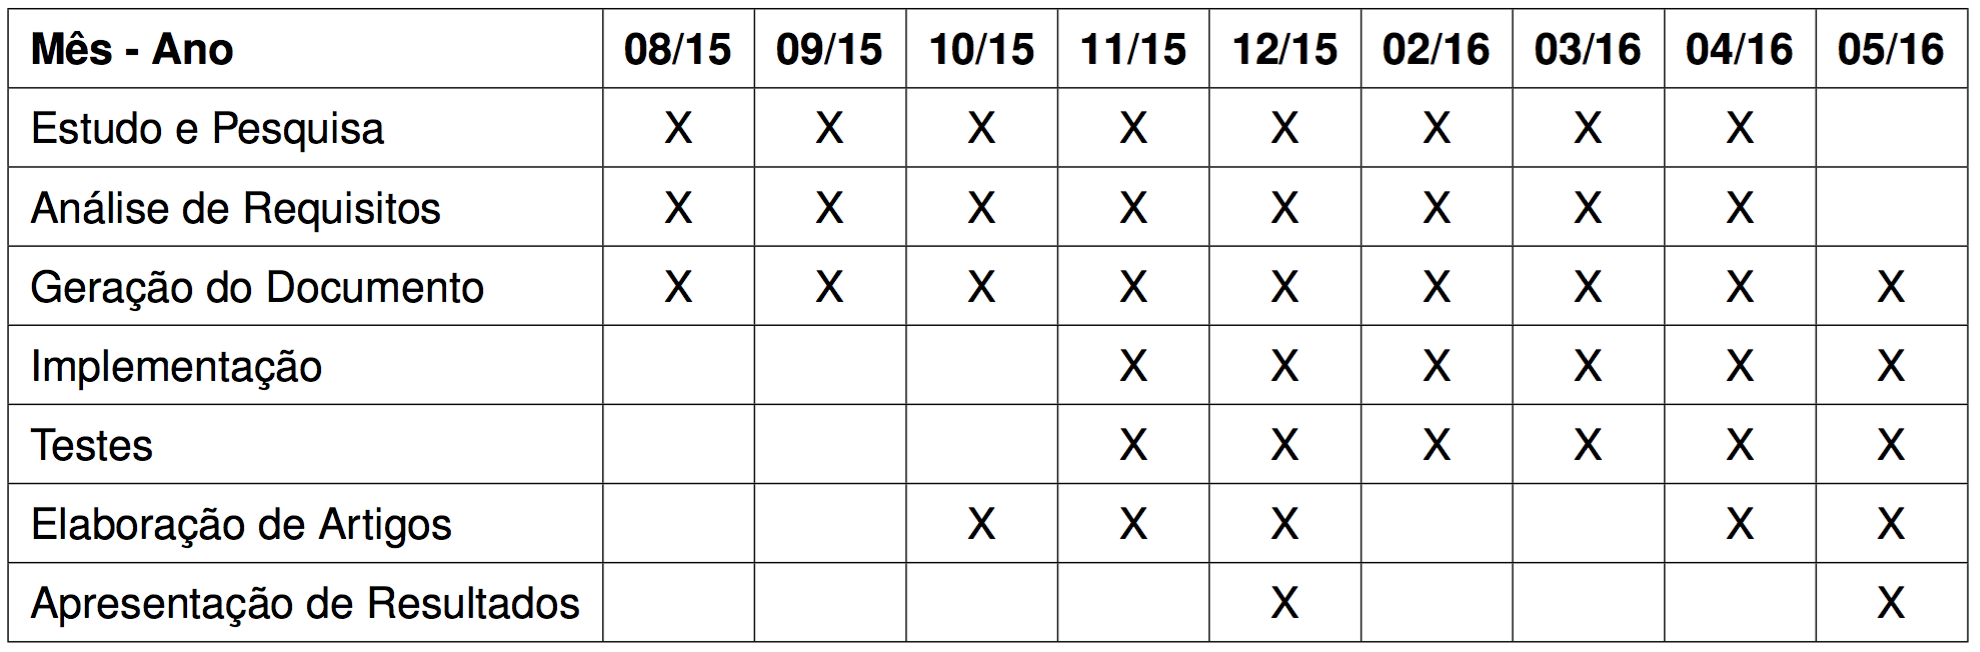
\includegraphics[width=1\textwidth]{tabela}
	\fonte{Autor}
	\label{crono}
\end{table}

\begin{itemize}
  \item Estudo e Pesquisa: aquisição dos conhecimentos pertinentes e necessários para o desenvolvimento do projeto;
  \item Análise de Requisitos: levantamento dos requisitos do projeto;
  \item Geração do Documento: desenvolvimento das documentações para especificação do projeto;
  \item Implementação: desenvolvimento dos códigos para a análise de dados;
  \item Testes: execução dos testes que irão garantir a qualidade das informações a serem geradas;
  \item Elaboração de Artigos: parte do tempo destinado ao projeto será para desenvolver artigos visando a publicação em eventos da área;
  \item Apresentação de Resultados: etapas destinadas à apresentação dos resultados parciais e finais.
\end{itemize}



\begin{table}[h!]
	\centering
	\caption{Cronograma de execução}
	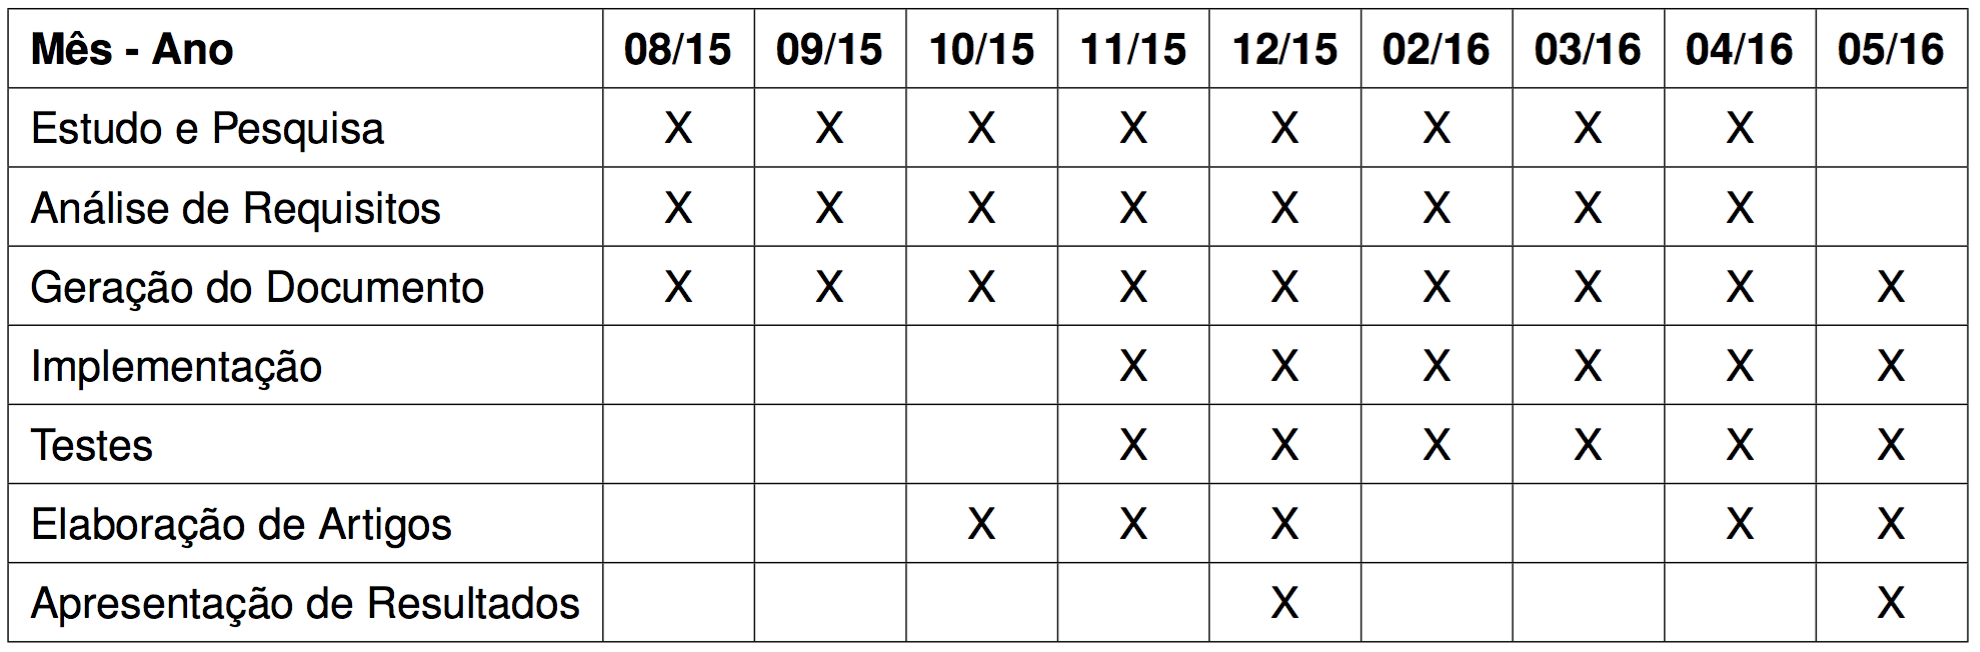
\includegraphics[width=1\textwidth]{tabela}
	\fonte{Autor}
	\label{cronograma}
\end{table}


\section{ORGANIZAÇÃO DO TRABALHO}\label{sec:organizacao-trabalho}

Além deste capítulo \autoref{crono}, este trabalho é composto de mais seis capítulos.

O Capítulo 2 apresenta os trabalhos que são referências para este estudo.

Os fundamentos teóricos, como os conceitos de \textit{data mining} e base para o entendimento do tema proposto, estão descritos no Capítulo 3.

No Capítulo 5 são apresentadas as fases do desenvolvimento ....

Os resultados obtidos e a apresentação de planilhas e gráficos das soluções desenvolvidas são apresentados no Capítulo 6.

Por fim, a conclusão deste trabalho se dá no Capítulo 7, onde são abordadas e analisadas as dificuldades, além de determinar as possibilidades para trabalhos futuros.
